\documentclass[12pt, a4paper, oneside]{ctexart}
\usepackage{amsmath, amsthm, amssymb, bm, color, graphicx, geometry, mathrsfs,extarrows, braket, booktabs, array}
\usepackage[colorlinks,linkcolor=red,anchorcolor=blue,citecolor=blue,urlcolor=blue,menucolor=black]{hyperref}
%%%% 设置中文字体 %%%%
\setCJKmainfont{方正新书宋_GBK.ttf}[BoldFont=方正小标宋_GBK, ItalicFont=方正楷体_GBK]
%%%% 设置英文字体 %%%%
\setmainfont{Times New Roman}
\setsansfont{Calibri}
\setmonofont{Consolas}

\linespread{1.4}
%\geometry{left=2.54cm,right=2.54cm,top=3.18cm,bottom=3.18cm}
\geometry{left=1.84cm,right=1.84cm,top=2.18cm,bottom=2.18cm}
\newcounter{problem}  % 问题序号计数器
\newenvironment{problem}{\stepcounter{problem}\par\noindent\textbf{题目\arabic{problem}. }}{\smallskip\par}
\newenvironment{solution}[1][]{\par\noindent\textbf{#1解答. }}{\smallskip\par}  % 可带一个参数表示题号\begin{solution}{题号}
\newenvironment{note}{\par\noindent\textbf{注记. }}{\smallskip\par}

%%%% 图片相对路径 %%%%
% \graphicspath{{figure/}} % 当前目录下的figure文件夹, {../figure/}则是父目录的figure文件夹
\setlength{\abovecaptionskip}{-0.2cm}  % 缩紧图片标题与图片之间的距离
\setlength{\belowcaptionskip}{0pt} 

\everymath{\displaystyle} % 默认全部行间公式
\DeclareMathOperator*\uplim{\overline{lim}} % 定义上极限 \uplim_{}
\DeclareMathOperator*\lowlim{\underline{lim}} % 定义下极限 \lowlim_{}
\DeclareMathOperator*{\argmax}{arg\,max}  % \argmin
\DeclareMathOperator*{\argmin}{arg\,min}  % \argmax
\let\leq=\leqslant % 将全部leq变为leqslant
\let\geq=\geqslant % geq同理

%%%% 一些宏定义 %%%%
\def\bd{\boldsymbol}        % 加粗(向量) boldsymbol
\def\disp{\displaystyle}    % 使用行间公式 displaystyle(默认)
\def\tsty{\textstyle}       % 使用行内公式 textstyle
\def\sign{\text{sign}}      % sign function
\def\wtd{\widetilde}        % 宽波浪线 widetilde
\def\R{\mathbb{R}}          % Real number
\def\N{\mathbb{N}}          % Natural number
\def\Z{\mathbb{Z}}          % Integer number
\def\Q{\mathbb{Q}}          % Rational number
\def\C{\mathbb{C}}          % Complex number
\def\N{\mathbb{N}}          % Natural number
\def\Z{\mathbb{Z}}          % Integer number
\def\d{\mathrm{d}}          % differential operator
\def\e{\mathrm{e}}          % Euler's number
\def\i{\mathrm{i}}          % imaginary number
\def\re{\mathrm{Re}}        % Real part
\def\im{\mathrm{Im}}        % Imaginary part
\def\res{\mathrm{Res}}      % Residue
\def\L{\mathcal{L}}         % Loss function
\def\wdh{\widehat}          % 宽帽子 widehat
\def\ol{\overline}          % 上横线 overline
\def\ul{\underline}         % 下横线 underline
\def\add{\vspace{1ex}}      % 增加行间距
\def\del{\vspace{-3.5ex}}   % 减少行间距

%%%% 定理类环境的定义 %%%%
\newtheorem{theorem}{定理}

%%%% 基本信息 %%%%
\newcommand{\RQ}{\today} % 日期
\newcommand{\km}{数学建模} % 科目
\newcommand{\bj}{强基数学002} % 班级
\newcommand{\xm}{吴天阳} % 姓名
\newcommand{\xh}{2204210460} % 学号

\begin{document}

%\pagestyle{empty}
\pagestyle{plain}
\vspace*{-15ex}
\centerline{\begin{tabular}{*5{c}}
    \parbox[t]{0.25\linewidth}{\begin{center}\textbf{日期}\\ \large \textcolor{blue}{\RQ}\end{center}} 
    & \parbox[t]{0.2\linewidth}{\begin{center}\textbf{科目}\\ \large \textcolor{blue}{\km}\end{center}}
    & \parbox[t]{0.2\linewidth}{\begin{center}\textbf{班级}\\ \large \textcolor{blue}{\bj}\end{center}}
    & \parbox[t]{0.1\linewidth}{\begin{center}\textbf{姓名}\\ \large \textcolor{blue}{\xm}\end{center}}
    & \parbox[t]{0.15\linewidth}{\begin{center}\textbf{学号}\\ \large \textcolor{blue}{\xh}\end{center}} \\ \hline
\end{tabular}}
\begin{center}
    \zihao{3}\textbf{第二次作业}
\end{center}\vspace{-0.2cm}
\begin{problem}
    医生给病人开处方时必须注明两点:服药的剂量和服药的时间间隔.超剂量的药品会对身体产生严重不良后果,甚至死亡,而剂量不足,则不能达到治病的目的.已知患者服药后,随时间推移,药品在体内\textbf{逐渐被吸收},发生生化反应,也就是体内药品的浓度逐渐降低.\textbf{药品浓度降低的速率与体内当时药品的浓度成正比}.当服药量为$A$、\textbf{服药间隔}为$T$,试分析体内药的浓度随时间的变化规律.
\end{problem}
\begin{solution}
    设机体体积为$V$,药品分解系数为$k_1$,机体吸收系数为$k_2$,考虑第$n$次服药到$n+1$次服药时间段内药量的变化,即$(n-1)T\leq t < nT$,令$y_n(t),\ t\in[0,T]$表示第$n$个时间段内药物未分解的量(残量);$x_n(t),\ t\in[0,T]$为第$n$个时间段内已分解的药物量(分解但未被机体吸收),则有以下方程成立
    \begin{equation*}
        \begin{cases}
            y_n' = -k_1y_n,\\
            y_n(0) = y_{n-1}(T)+A.
        \end{cases}
        \quad\begin{cases}
            x'_n=-k_2x_n+k_1y_n,\\
            x_n(0) = x_{n-1}(T).
        \end{cases}\text{且}\ x_0(T) = y_0(T) = 0.
    \end{equation*}
    解得当$n=1$时
    \begin{equation*}
        y_1 = A\e^{-k_1t},\quad x_1=\frac{k_1A}{k_2-k_1}(\e^{-k_1t}-\e^{-k_2t}),
    \end{equation*}
    当$n\geq 2$时
    \begin{equation*}
        y_n = y_{n-1}(T)\e^{-k_1t}+A\e^{-k_1t},\quad x_n=\frac{k_1(y_{n-1}(T)+A)}{k_2-k_1}(\e^{-k_1t}-\e^{-k_2t})+x_{n-1}(T)\e^{-k_2t}.
    \end{equation*}
    通过迭代表达式易求$y_n$的显示表达式
    \begin{equation*}
        y_n = \frac{A\e^{k_1(T-t)}(1-\e^{-nk_1T})}{\e^{k_1T}-1}.
    \end{equation*}
    且可以发现当$n\to\infty$时$y_n$收敛,\add 记$y_n\to y$,则$y(t) = \frac{A\e^{k_1(T-t)}}{\e^{k_1T}-1}$且单调递减,则有$y(0) = \frac{A\e^{k_1T}}{\e^{k_1T}-1},\ y(T) = \frac{A}{\e^{k_1T}-1}$,所以最终药物残量维持在$\left[\frac{A}{\e^{k_1T}-1}, \frac{A\e^{k_1T}}{\e^{k_1T}-1}\right]$.\add

    而$x_n$显示表达式较难求解,我们考虑求解$n\to\infty$时的解. 假设$x_n$收敛于$x$,由递推式可知
    \begin{equation}
        x(t)=\frac{k_1}{k_2-k_1}(y(T)+A)(\e^{-k_1t}-\e^{-k_2t})+x(T)\e^{-k_2t},
    \end{equation}
    取$t=T$可得
    \begin{align*}
        &\ x(T) = \frac{k_1}{k_2-k_1}(y(T)+A)(\e^{-k_1T}-\e^{-k_2T})+x(T)\e^{-k_2T}\\
        \Rightarrow&\ x(T) = \frac{k_1}{k_2-k_1}\,\frac{A(\e^{k_2T}-\e^{k_1T})}{(\e^{k_1T}-1)(\e^{k_2T}-1)},
    \end{align*}
    带回到(1)式中有
    \begin{align*}
        x(t) =&\ \frac{k_1}{k_2-k_1}\,\frac{A\e^{k_1T}}{\e^{k_1T}-1}(\e^{-k_1t}-\e^{-k_2t})+\frac{k_1}{k_2-k_1}\,\frac{A(\e^{k_2T}-\e^{k_1T})}{(\e^{k_1T}-1)(\e^{k_2T}-1)}\e^{-k_2t}\\
        &\ = \frac{k_1A}{k_2-k_1}\left(\frac{\e^{k_1(T-t)}}{\e^{k_1T}-1}-\frac{\e^{k_2(T-t)}}{\e^{k_2T}-1}\right).
    \end{align*}
    则$x(0) = \frac{k_1}{k_2-k_1}\,\frac{A(\e^{k_2T}-\e^{k_1T})}{(\e^{k_1T}-1)(\e^{k_2T}-1)} = x(T)$,所以当时间充分长时,每两次服药时,机体内药物浓度相同.

    下面求解$x(t)$的最大值,先求最值点
    \begin{equation*}
        x'(t_0) = 0\Rightarrow t_0 = T -\frac{1}{k_2-k_1}\log\frac{k_1(\e^{k_2T}-1)}{k_2(\e^{k_1T}-1)},
    \end{equation*}
    于是最大值为
    \begin{equation*}
        x(t_0) = \frac{k_1A}{k_2-k_1}\left(\left(\frac{k_1}{k_2}\right)^{\frac{k_1}{k_2-k_1}}-\left(\frac{k_1}{k_2}\right)^{\frac{k_2}{k_2-k_1}}\right)\frac{(\e^{k_2T}-1)^{\frac{k_1}{k_2-k_1}}}{(\e^{k_1T}-1)^{\frac{k_2}{k_2-k_1}}}.
    \end{equation*}
    所以$\forall k_1,k_2,T,A$,机体内的药物浓度都具有上界,而不是无限增长的.

    下面用程序对上述估计结果进行验证,取$k1=1,k2=0.5,A=10,T=1$,服用$30$个周期,得到如下结果
    \begin{figure}[htbp]
        \centering
        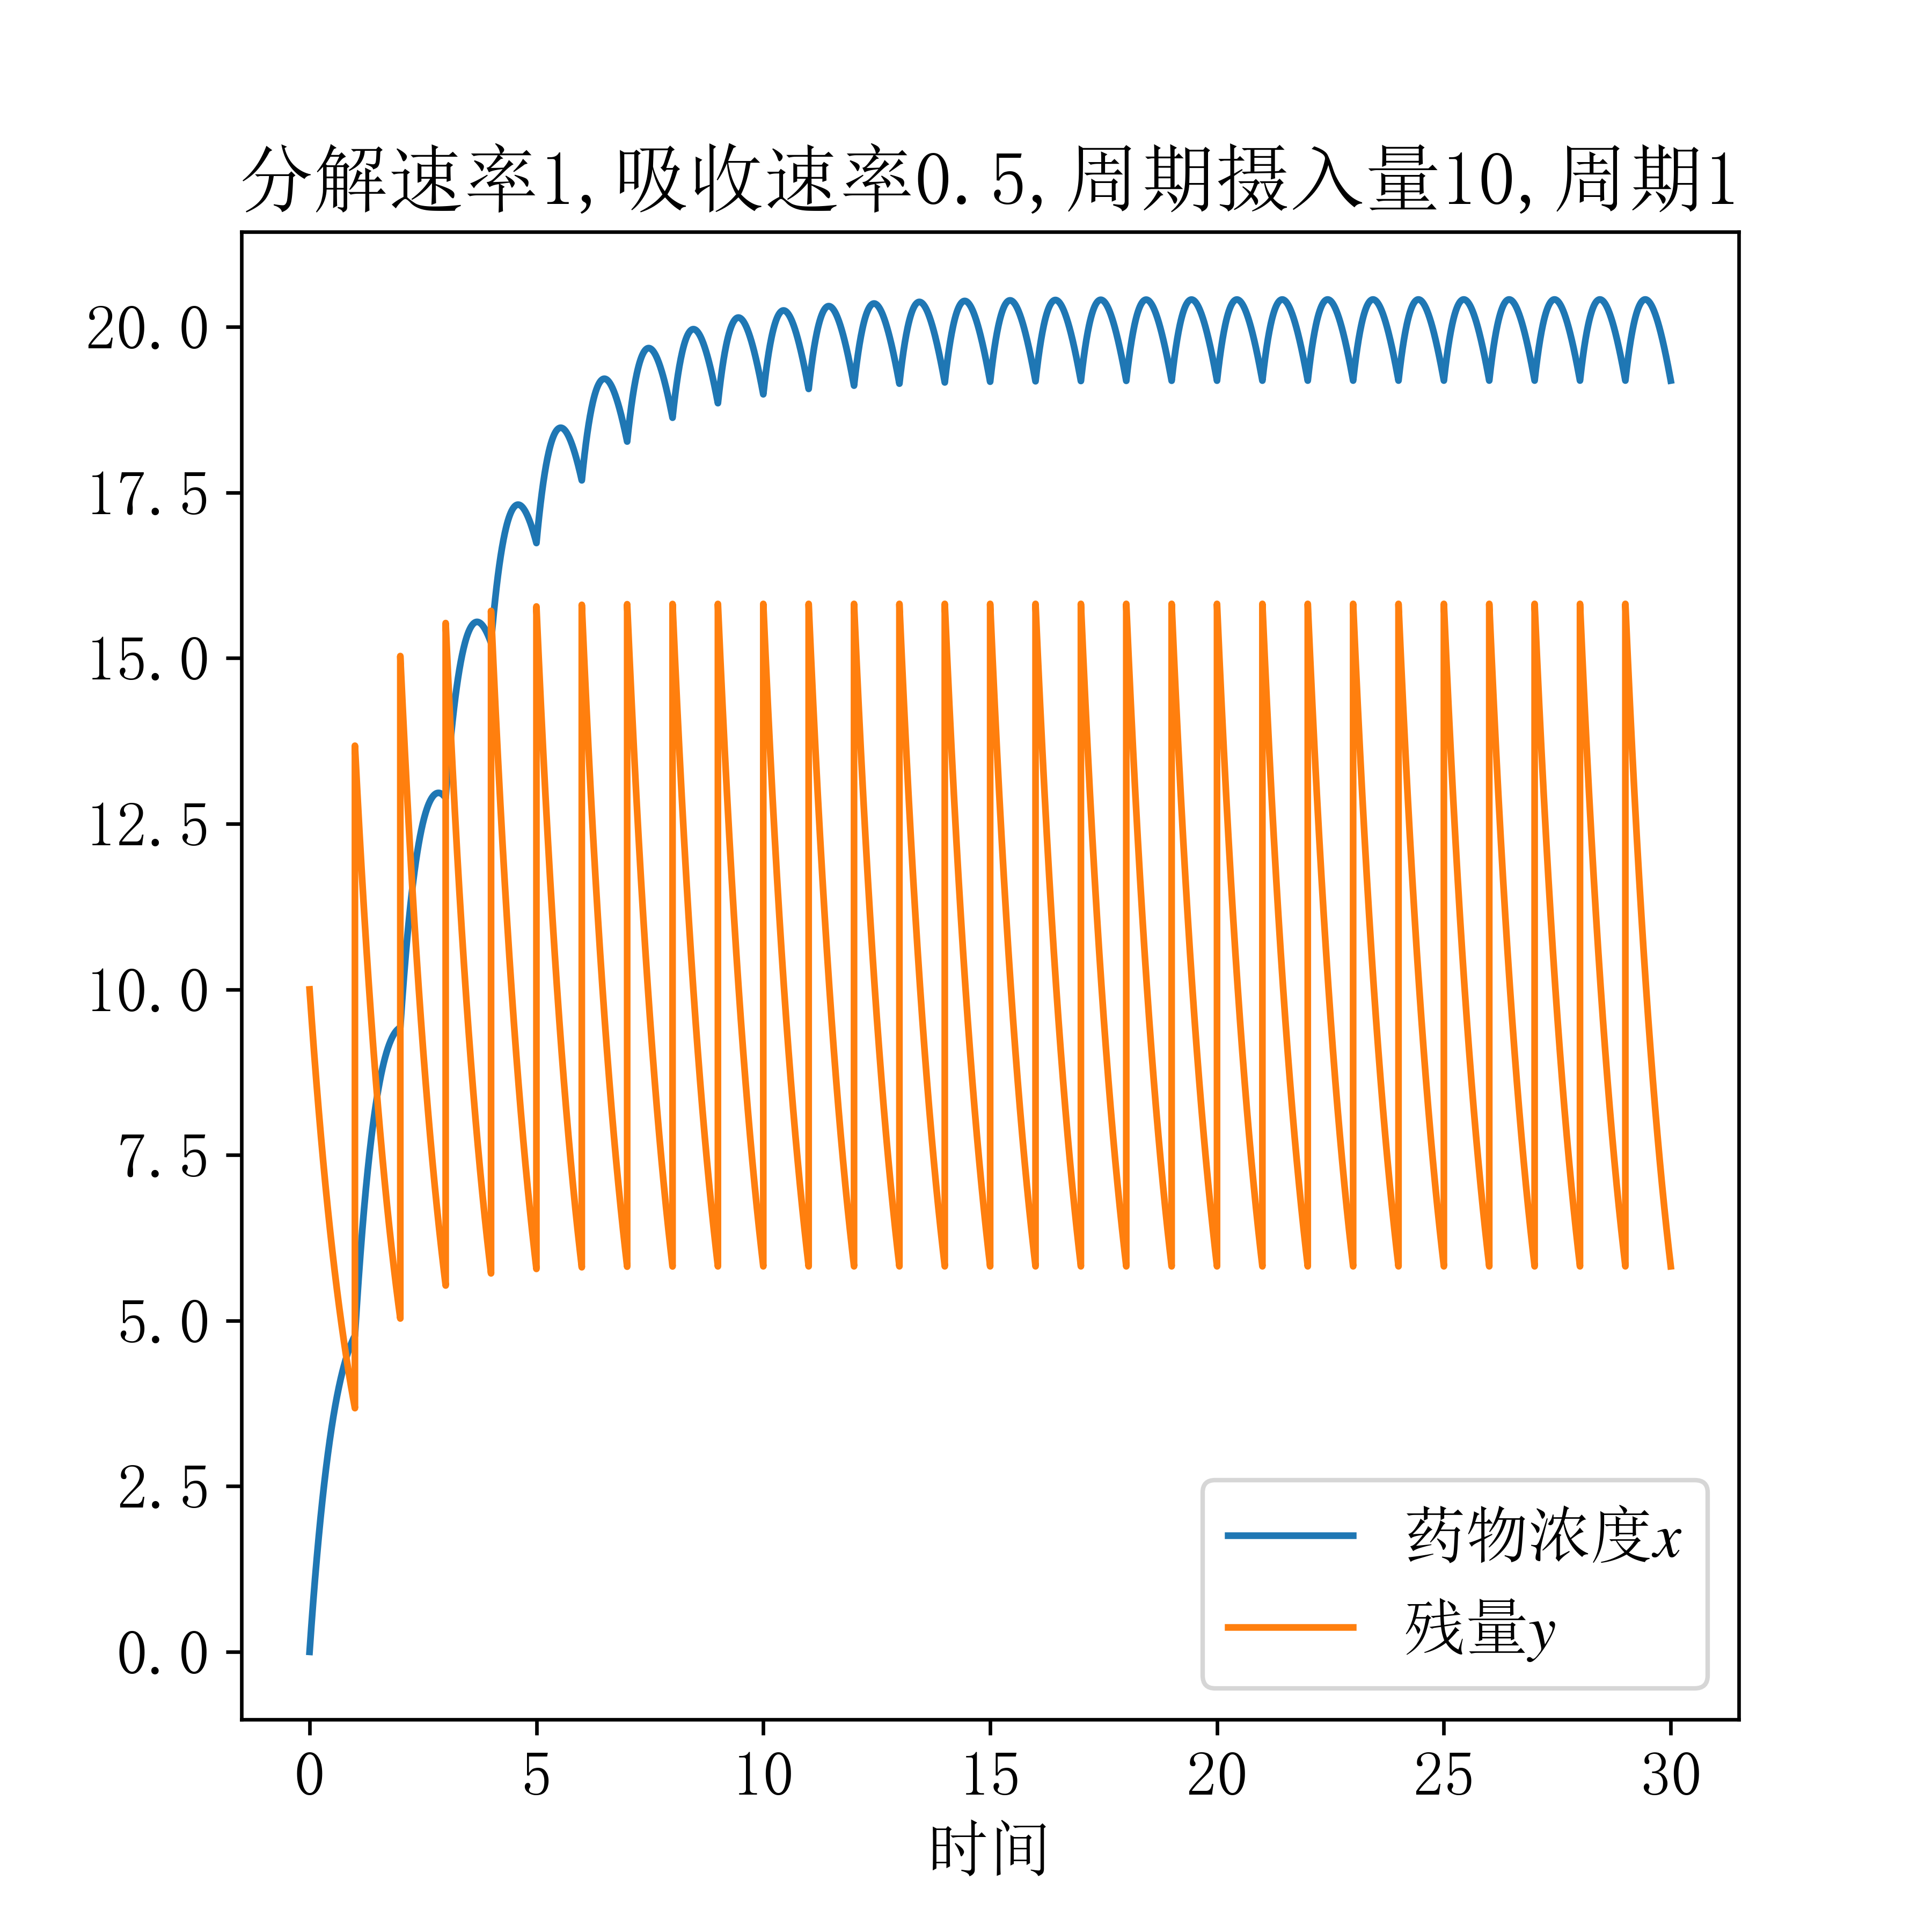
\includegraphics[scale=0.8]{浓度与残量关于时间变化关系.png}
    \end{figure}

    \par\noindent 实际值:$x(0)=19.190338082418194, y(0)=5.8197670686927, x_{max}=20.414854591829517$\\
    估计值:$x(0)=19.190347513349437, y(0)=5.8197670686933, x_{max}=20.414940825367978$.
\end{solution}

% 正文部分

% 下面给一些功能的写法
\iffalse
% 图片模板
\centerline{
    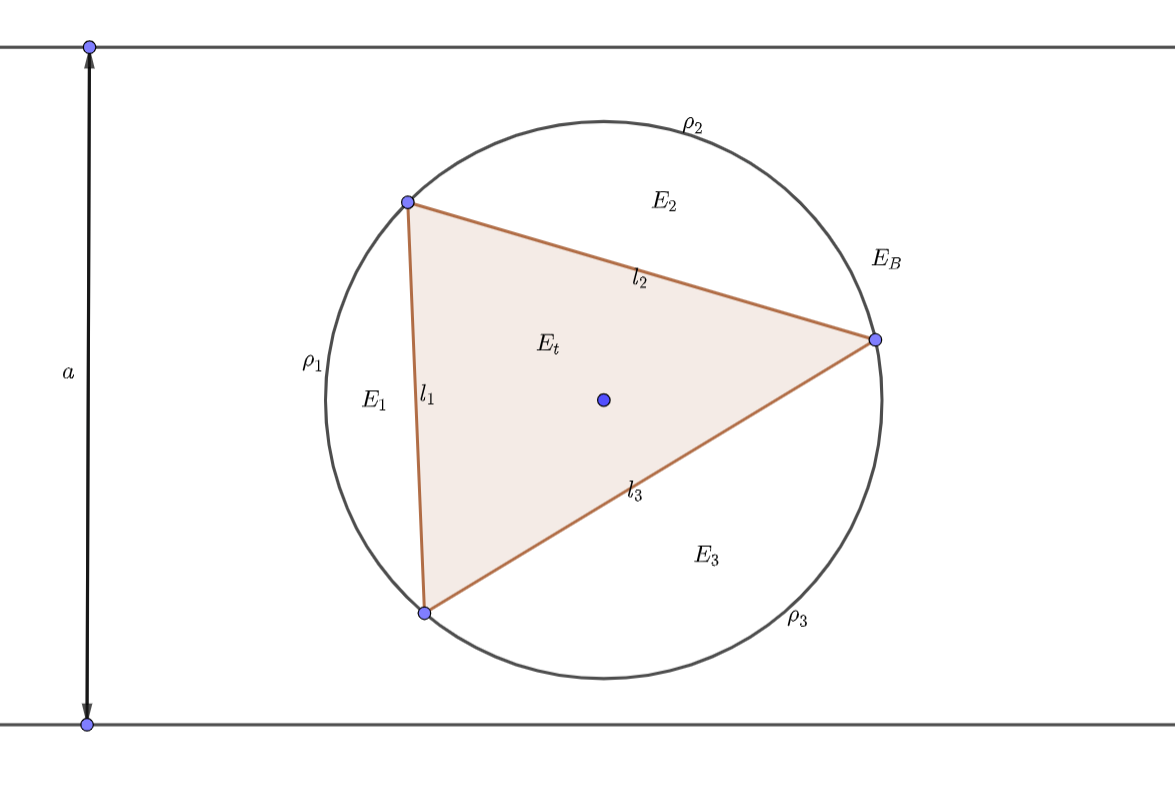
\includegraphics[width=0.8\textwidth]{figure.png}
}
% 表格模板
\renewcommand\arraystretch{0.8} % 设置表格高度为原来的0.8倍
\begin{table}[!htbp] % table标准
    \centering % 表格居中
    \begin{tabular}{p{1cm}<{\centering}p{1cm}<{\centering}p{3cm}<{\centering}p{5cm}<{\centering}} % 设置表格宽度
    %\begin{tabular}{cccc}
        \toprule
        $x_i$ & $f[x_1]$ & $f[x_i,x_{i+1}]$ & $f[x_i,x_{i+1},x_{i+2}]$ \\
        \midrule
        $x_0$ & $f(x_0)$ &                  &                          \\
        $x_0$ & $f(x_0)$ & $f'(x_0)$        &                          \\
        $x_0$ & $f(x_1)$ & $\frac{f(x_1)-f(x_0)}{x_1-x_0}$ & $\frac{f(x_1)-f(x_0)}{(x_1-x_0)^2}-\frac{f'(x_0)}{x_1-x_0}$\\
        \bottomrule
    \end{tabular}
\end{table}

\def\Log{\text{Log}} % 一个简单的宏定义
$\Log$ % 调用方法
\fi

\end{document}